% Slides for 2024-05-06
% To create a slide, use the following:
% \begin{frame}{TITLE}
%     BODY
% \end{frame}

% To create a slide with a bullet list, use the following:
% \begin{frame}{TITLE}
%     \begin{itemize}
%         \item ITEM 1
%         \item ITEM 2
%     \end{itemize}    
% \end{frame}

% To create a slide with numbered list, use the following:
% \begin{frame}{TITLE}
%     \begin{enumerate}
%         \item ITEM 1
%         \item ITEM 2
%     \end{enumerate}
% \end{frame}

% To create a slide with a graphic:
% 1. Add the graphic to this folder (named picture.png)
% 2. Use the following:
% \begin{frame}{TITLE}
%     \centering
%     \includegraphics[height=0.7\textheight,width=0.7\textwidth,keepaspectratio]{picture.png}
% \end{frame}

% To create a slide with two columns, use the following:
% \begin{frame}{TITLE}
%     \begin{columns}
%         \begin{column}{0.5\textwidth}
%             COLUMN 1 BODY
%         \end{column}
%         \begin{column}{0.5\textwidth}
%             COLUMN 2 BODY
%         \end{column}
%     \end{columns}
% \end{frame}


\begin{frame}{Rust Backend - In Progress}
    \begin{columns}
        \begin{column}{0.5\textwidth}
            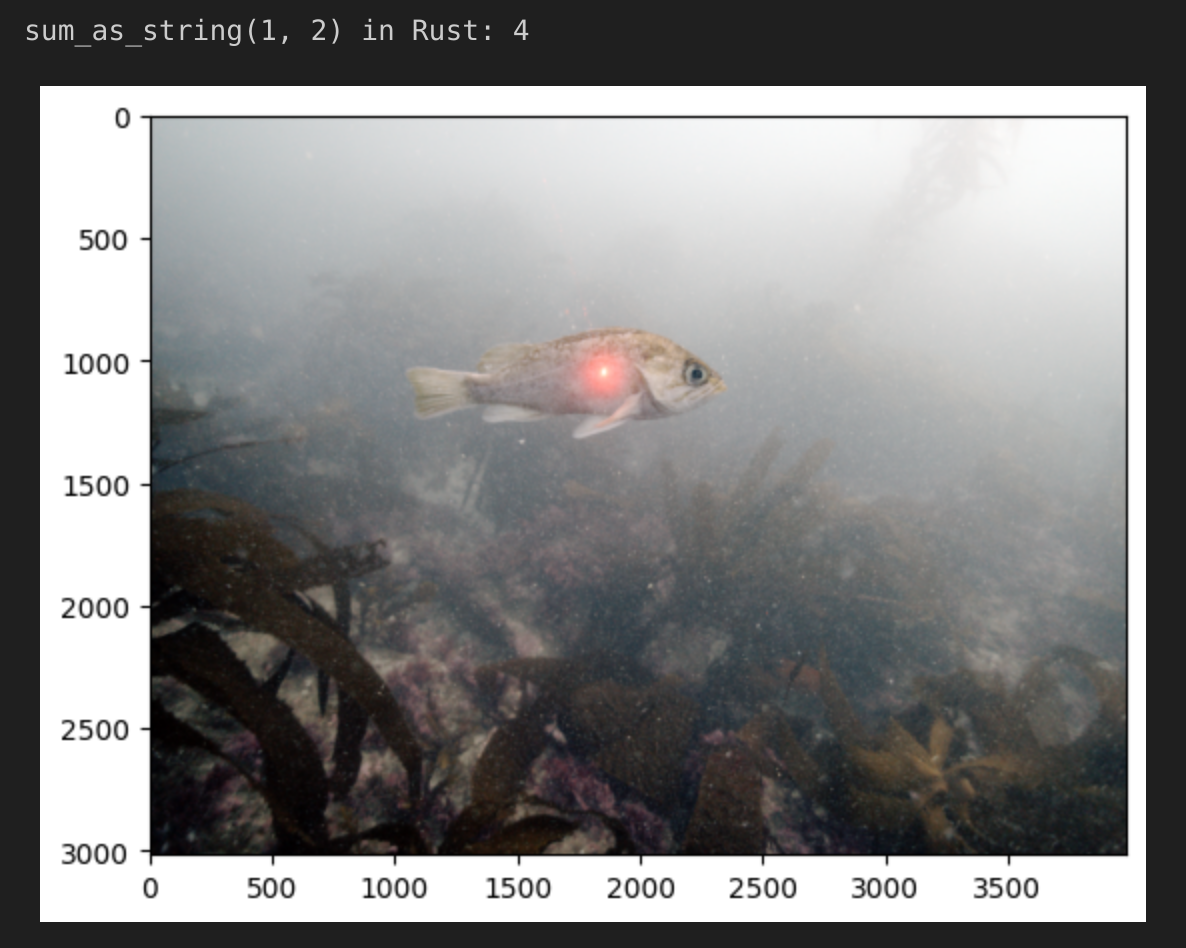
\includegraphics[height=0.7\textheight,width=0.7\textwidth,keepaspectratio]{images/fs_cli_rust.png}
        \end{column}
        \begin{column}{0.5\textwidth}
            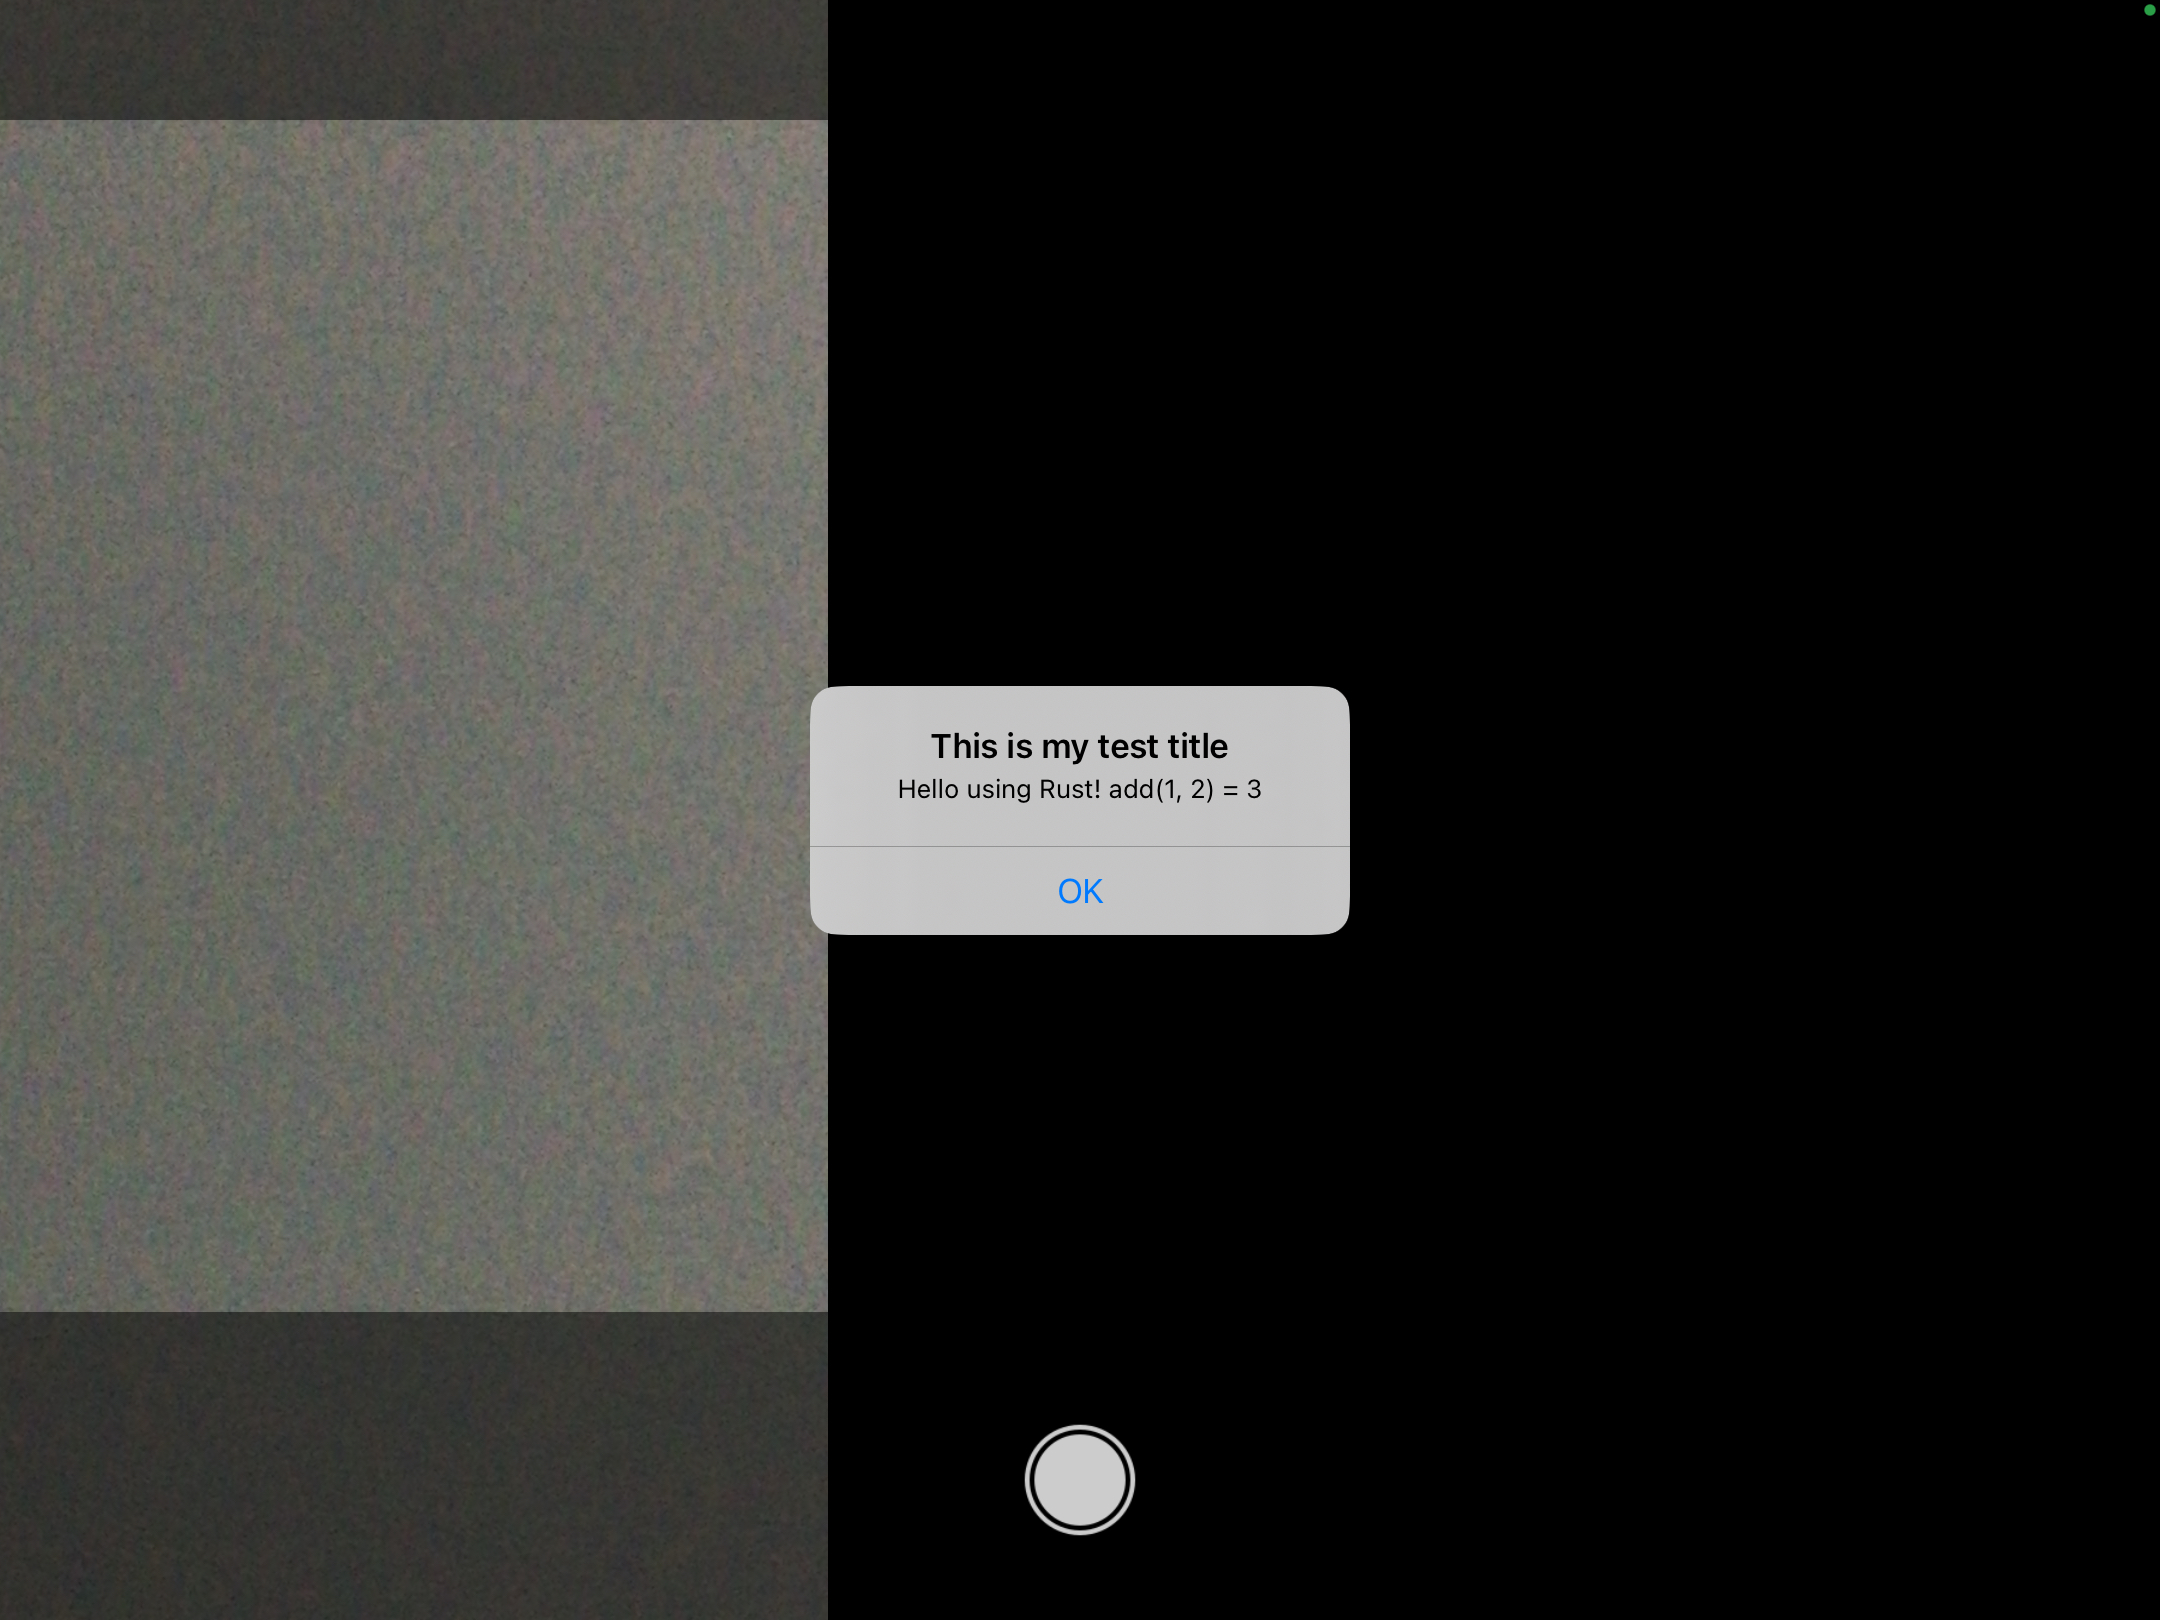
\includegraphics[height=0.7\textheight,width=0.7\textwidth,keepaspectratio]{images/fs_ipad_rust.png}
        \end{column}
    \end{columns}
\end{frame}

\begin{frame}{CA Cares}
    \begin{enumerate}
        \item Submission Delayed - May 10
        \item In Person Team Connection - Thursday
    \end{enumerate}
\end{frame}

\begin{frame}{SCCOOS}
    Poster session on 5/14-5/16
\end{frame}

\begin{frame}{NISEC}
    Four slide presentation - Should I put one together?
\end{frame}

\begin{frame}{SDIC Showcase - Due Today!}
    Should we apply?: https://sdic.org/2024-showcase2024/
\end{frame}